\section{Merkle Hash Trees}

Let \[h: \Omega^\ast \rightarrow \Omega^l\]
be a cryptographic hash function for an alphabet \(\{0,1\} \subseteq \Omega\) %, e.g.\
%\(\Omega = \{0,1\}\) 
and a fixed natural number \(0 < l \in \N\).
\((\Omega^\ast, +, \epsilon)\) is the semigroup of words of
\(\Omega\) with concatenation \(+\) and zero element \(\epsilon\).
The results are often called hash values or message digest or
simply digest.

Cryptographic hash functions share the following properties:
\begin{itemize}
\item \emphind{Pre-image resistance}: It is difficult to find a
pre-image. (One-way-function)
\item \emphind{Second pre-image resistance}: Given an \(m_1 \in \Omega^\ast\)
is difficult to find a \(m_2 \ne m_1 \in   \Omega^\ast\) such that
\(h(m_1) = h(m_2)\).
\item \emphind{Collision resistance}: It is difficult to find \(m_1 \ne m_2 \in   \Omega^\ast\)
such that \(h(m_1) = h(m_2)\).
\end{itemize}
Furthermore, we have a finite sequence 
\[d := (d_0,\ldots,d_{n-1}) = (d_i)_{0 \le i < n} \in {\Omega^\ast}^n\]
of messages or documents
for \(0 \le n \in \N\).

\begin{definition}
A Merkle hash tree \(t_h(d)\) for \(h\) and \(d\) is defined recursively to 
have its nodes labelled by
\begin{itemize}
\item \(M(d) := h(\epsilon)\), if \(d\) is the empty list for \(n=0\)
and the empty word \(\epsilon \in \Omega^\ast\) (empty list),
\item \(M((d_0)) := h(d_0)\) for \(d = (d_0)\) is a one-element
list, i.e.\ \(n = 1\) (leaf) and finally
\item for \(n > 1\) we define \(k \in \N\) to 
be the largest power of 2 smaller than \(n\), i.e.
\(k < n \le 2k\) we set
\[M((d)) := h(M((d_i)_{0 \le i < k}+M( (d_i)_{k \le i < n})\].
\end{itemize}
Note, that it is a binary tree.
\end{definition}
Note, that the authors of \cite{LLK2013} use SHA-256 for \(h\) an require
additional concatenations of 00 resp.\ 01 from the left \(M((d_0)) := h(00+d_0)\) and
\(M((d)) := h(01+M((d_i)_{0 \le i < k}+M( (d_i)_{k \le i < n})\). The purpose
for that is not yet clear. They claim, that adding 00 from left to a leaf node
and 01 for the other nodes is required to give second preimage resistance.
 
All the nodes of the Merkle binary tree are labelled by hashes. The tree
has \(n\) leaves labelled by the hashes \((h(d_i))_{0 \le i < n}\).
Merkle trees do not have to have the same depth for their leaves, i.e.\
distances from the root. But the number \(n\) of leaves determines
the shape of the tree. If  \(n = 2^\kappa\) is a power of 2, then 
we have the perfect binary tree of depth \(\kappa\). 
Otherwise, we
assume that \(k=2^\kappa < n \le 2^{\kappa+1}\), then the tree shape is
recursively determined by the root node with the perfect binary
tree of depth \(\kappa\) as left child and the binary tree with
the shape of the binary tree with \(n-k\) leaves as right child.
Labelling edges to left children with 0 and those to right children
with 1 the path from the root to the \(i\)-th leave \(0 \le i < n\)
is the binary expansion of \(i\), provided we fill binary path words 
of length smaller than \(k+1\) with zeros to the right.

\subsection{Paths in Merkle Trees}

\begin{lemma}
Let \(t\) a Merkle tree for the leaves \(d = (d_i)_{0 \le i < n}\). The path from 
the root of \(t\) to 
the \(i\)-th leaf \(d_i\), \(0 \le i < n\) is given by 
an element \(p(i) \in \{0,1\}^\ast\) of length equal or smaller to the maximal depth 
\(\kappa\) of the tree, given by 
\(2^\kappa < n \le 2^{\kappa+1}\).
Then the path is given by interpreting \(p(i)\) form left
to right, where 0 moves to the left
child, while 1 moves to the right child. 

The word \(p(i)\) is constructed as follows: Add leading 0's to the 
binary expansion \((i_{\kappa-1},\ldots,i_1,i_0)_2 = i_{10}\) with
length \(\kappa\). Drop the last zeros, if the leaf is reached in less
than \(\kappa\) steps. Note, that this only can happen for \(i=n-1\).
\end{lemma}
\begin{proof}
By the construction of the Merkle tree from its leaves
it is clear that the first \(\lceil\frac{m}{2}\rceil\)
leaves are paired in the first step and hence will have maximal depth.
In case of an odd \(m\) the Euclidean algorithm for \(m-1\)
and 2 gives 0's as long as the hash of the last leaf can not be paired, i.e.\
the path for this leave must be shortened by the rightmost 0's.
\end{proof}
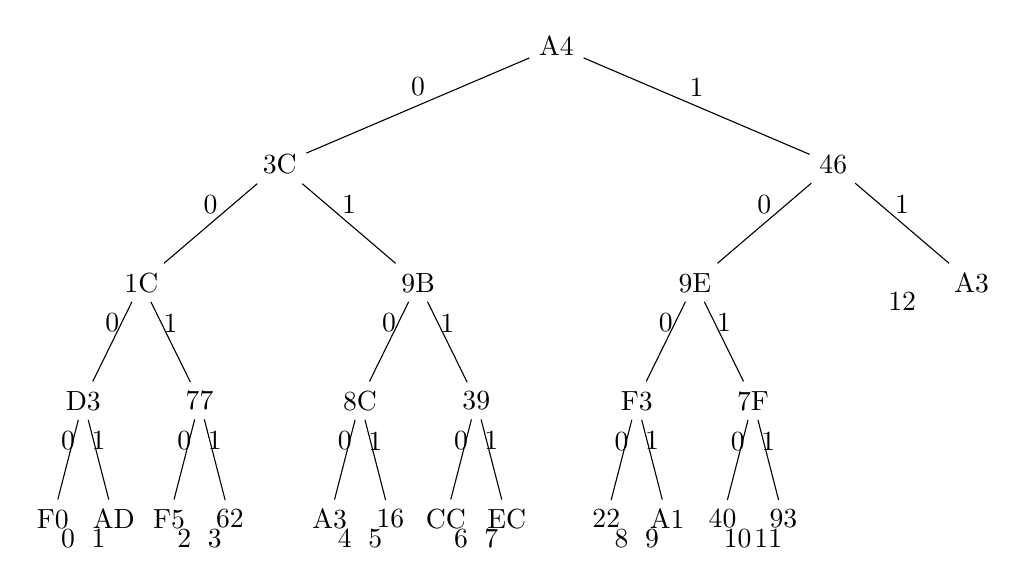
\begin{tikzpicture}[
  level 1/.style={sibling distance=20em},
  level 2/.style={sibling distance=10em},
  level 3/.style={sibling distance=4.2em},
  level 4/.style={sibling distance=2.2em}, 
  ]
  \node {A4}
    child { node  {3C} 
      child { node  {1C} 
        child { node  {D3}
          child { node (0)  {F0} 
            edge from parent node[above] {0} 
    	    node [below of = 0] {0}
          }
          child { node  {AD}
            edge from parent node[above] {1} 
    	    node [below of = 0] {1}
	  }
          edge from parent node[above] {0} 
        }
        child { node  {77}
          child { node  {F5} 
            edge from parent node[above] {0} 
    	    node [below of = 0] {2}
          }
          child { node  {62} 
            edge from parent node[above] {1} 
    	    node [below of = 0] {3}
          }
          edge from parent node[above] {1} 
        }
        edge from parent node[above] {0} 
      } 
      child { node  {9B} 
        child { node  {8C}
          child { node  {A3} 
            edge from parent node[above] {0} 
    	    node [below of = 0] {4}
          }
          child { node  {16} 
            edge from parent node[above] {1} 
    	    node [below of = 0] {5}
          }
          edge from parent node[above] {0} 
        }
        child { node  {39}
          child { node  {CC} 
            edge from parent node[above] {0} 
    	    node [below of = 0] {6}
          }
          child { node  {EC} 
            edge from parent node[above] {1} 
    	    node [below of = 0] {7}
          }
          edge from parent node[above] {1} 
        }
        edge from parent node[above] {1} 
      }
      edge from parent node[above] {0} 
    } 
    child { node  {46} 
      child { node  {9E} 
        child { node  {F3}
          child { node  {22} 
            edge from parent node[left, above] {0} 
    	    node [below of = 0] {8}
          }
          child { node  {A1} 
            edge from parent node[right, above] {1} 
    	    node [below of = 0] {9}
          }
          edge from parent node[above] {0} 
        }
        child { node  {7F}
          child { node  {40} 
            edge from parent node[above] {0} 
    	    node [below of = 0] {10}
          }
          child { node  {93} 
            edge from parent node[above] {1} 
    	    node [below of = 0] {11}
          }
          edge from parent node[above] {1} 
        }
        edge from parent node[above] {0} 
      }
      child { node  {A3} 
        edge from parent node[above] {1} 
    	node [below of = 0] {12}
      } 
      edge from parent node[above] {1} 
    }; 
\end{tikzpicture}


\subsection{Notation in Merkle Trees}
For a node \(\nd\) in a Merkle hash tree we denote
by \(\nd.h\) its hash, by \(\nd.l\) its left child, 
by \(\nd.r\) its right child and by 
\(\nd.p\) its parent node. Note, that for a leaf
node we have \(\nd.l = \nd.r = []\), the empty tree
as well for the root node \(\nd.p = []\).


\section{Audit Proofs for Leaves}

\begin{definition}
For \(n > 1\) let \(k := 2^\kappa\) be the largest 
power of 2 such that \(k < n\). The \emphind{Merkle audit path} \(p(m, d)\) for 
the \(m+1\)-st element \(d_m\) in the list \(d = (d_i)_{0 \le i < n}\)
with \(0 \le m < n\) is recursively defined to be 
\begin{itemize}
\item \(p(0,(d_0)) := []\) for a single leaf in a tree with a one-element
input list;
\item \(p(m,d) := p(m, (d_i)_{0 \le i < k}) : M( (d_i)_{k \le i < n} )\) for \(m < k\) and
\item \(p(m,d) := p(m-k, (d_i)_{k \le i < n}) : M( (d_i)_{0 \le i < k})  \). 
\end{itemize}
Here \(:\) denotes the extension of a list by a further value.
\end{definition}
Note, that the audit path consists of the list of missing
nodes required to compute the nodes leading from 
a leaf to the root of the tree.
This can be used as a proof that the leaf exists in the tree by the 
properties of the cryptographic hash function \(h\):
\begin{theorem}
From \(p(m,d)\) and \(d_m\) for \(d = (d_i)_{0 \le i < n}\)
and \(0 \le m < n\) the hash \(M(d)\) can be 
computed by the following algorithm. 
Define \(k, \kappa \in \N\) such that \(k := 2^\kappa < n \le 2k = 2^{\kappa+1}.\)
Let \(m' := (m_\kappa,m_{\kappa-1},\ldots m_1,m_0)_2\) be the binary
expansion of \(m\), prolonged by leading 0's, if the length
is smaller than the length of the proof, by dropping final 0's, if the
length is larger.
\begin{itemize}
\item \(y := d_m\).
\item for \(p\) in \(p(m,d)\) and parallel for \(b\) in reverse \(m'\) repeat
	\begin{itemize}
		\item if \(b=1\) then \(y := h(p,y)\)
		\item else \(y := h(y, p)\)
	\end{itemize}
\item \(y = M(d)\).
\end{itemize}
\end{theorem}
\begin{proof}
If \(n=1\) then \(m=0\) and clearly \(M((d_0)) = h(d_0)\).
\((d)_{0 \le i < n})\) and the hash \(M((d_i)_{k \le i < n})\)
can be computed. But then the root hash of \(M(d)\) is the hash
of the concatenation of \(M((d_i)_{0 \le i < k})\) and \(M( (d_i)_{k \le i < n})\) 
for the case \(m < k\) and that of 
\(M((d_i)_{k \le i < n})\) and \(M( (d_i)_{0 \le i < k})\) by the
construction of the Merkle hash tree \(M(d)\).
\end{proof}

\section{Merkle Consistency Proof}
If we assume and want to guarantee that a Merkle hash tree can modified only by appending new leaves or 
further Merkle hash trees, it
is of utmost importance, that the owner of a document \(d_{m-1}\) who had received
the root hash \(M((d_i)_{0 \le i < m})\) of the Merkle hash tree after appending
the leaf \(h(d_{m-1})\) not only gets a confirmative yes that the subtree 
for the documents \(d' := (d_i)_{0 \le i < m}\)
is still unchanged and a part of the tree after 
further leaf extensions by \((d_i)_{m \le i < n} )\), but gets a proof of that.
If this tree still exists as a subtree node in the new tree for \(d := (d_i)_{0\le i < n}\)
the hash of the subtree for \(d'\) has changed. Hence, the owner should be provided
with a list of nodes
which enables him to compute \(M((d_i)_{0 \le i < n})\) as well
as to compute \(M((d_i)_{0 \le i < m})\), such that he compare the latter hash with 
originally given one for equality.

Hence, the task is the following
\begin{itemize}
\item 
Given  \(1 \le i \le m \le n\) and \(d := (d_0,d_1,\ldots,d_{n-1})\) and the 
Merkle tree \(t_h(d)\),
\item 
compute a list of hashes \(c(m,d)\) such that
\item
someone who knows \(m,n,M(d')\) and \(M(d)\)
\item
can compute both \(M(d')\) and \(M(d)\) and
from \(c(m,d)\) only using \(h\).
\end{itemize}

\begin{definition}
For \(1 \le m \le  n\), \(d := (d_i)_{0 \le i < n}\), 
and \(d' := (d_i)_{0 \le i < m}\) let \(k := 2^\kappa\) 
be the largest 
power of 2 such that \(k < n\). The Merkle consistency proof \(c(m, d)\) for 
the Merkle hash tree for \(d'\) with root hash \(M(d'\) to be a subtree of 
the Merkle hash tree for \(d\) with root hash \(M(d)\) is 
\[c(m,d) := c'(m,d,1),\]
where \(c'\)
is recursively defined to be 
\begin{itemize}
\item \(c'(m,d',1) := []\), if \(m=n\) and hence \(d=d'\), such that
the subtree coincides with the tree;
\item \(c'(m,d',0) := M(d)\), if \(m=n\) and hence \(d=d'\), such that 
the subtree coincides with the tree; 
\item \(c'(m,d,b) := c'(m, (d_i)_{0 \le i < k},b) : M( (d_i)_{k \le i < n})\) for \(m \le k\) and
\(b \in \{0,1\}\), note that the right subtree entries 
\((d_i)_{m \le i < n}\) only exist in the current tree;
\item \(c'(m,d,b) := c'(m-k, (d_i)_{k \le i < n},0) : M( (d_i)_{0 \le i < k})\) for \(m > k\) and
\(b \in \{0,1\}\), note that the left subtrees for \((d_i)_{0 \le i < k}\) have to be identical 
in both trees.  The number of nodes in the proof \(c(m,d)\) is bounded by \(\kappa + 1\).
\end{itemize}
Here \(:\) denotes the extension of a list by a further value.
\end{definition}

\begin{theorem}
The list \(c := c(m,d)\) can be used to computed \(r' := M(d',m)\) and \(r := M(d,m)\) by the following
algorithm.
\begin{itemize}
\item If \(m=n\) set \(lb\) to be the empty list. Compute the binary expansion of \(m-1\), extend to length \(\kappa\) by leading 0's, 
reserverse the order of the bits and drop the sequence of leading 1's. The result
is called \(lb\)
\item If \(m\) is a power of 2 or \(m = n\) set \(hx := r; hx' := r'\) 
\item else set \(hx := first c; hx' := first c, c := rest c\).
\item For \(u\) in c and for \(b\) in lb in parallel repeat
	\begin{itemize}
		\item if \(b=1\) then \(hx := h(u+hx); hx' := h(u+hx')\)
		\item else \(hx := h(hx+u\)
	\end{itemize}
\item \((hx' = r'\) and \((hx = r)\).
\end{itemize}
\end{theorem}
\begin{proof}
\begin{itemize}
\item
Let \(m = n\), then we have nothing to prove, as the two trees coincide. 
\item
Now we can assume that \(m < n\). As usual let \(k = 2^\kappa < n \le 2k = 2^{\kappa+1}\).
Two cases, namely \(m \le k\) and \(k < m\).
\item
If \(m \le k\) then \(h = h(r + last( c(m,d) ) ) \) else
\item 
case \(m > k\) then \(h( last( c(m,d) ) + r)\).

\item \(c'(m,d,b) := c'(m-k, (d_i)_{k \le i < n},0) : M( (d_i)_{0 \le i < k})\) for \(m > k\) and


\end{itemize}
\end{proof}


\subsection{Example of Consistency Proofs}

We define a list of 13 documents as the binary expansion of
\[(70293475092348750239478502934875^i)_{0 \le i < 13}.\]
After using the 512-bit padding of SHA-1 its hash codes
by SHA-1 are the following 7 40-digits hexadecimal numbers,
\scriptsize
\begin{center}
\texttt{F07F977DE683FCDB71347AF1E63FC039EF0F0074} \texttt{AD7D0CFE4CF22065EEC00AE5F9B3742A3F40C387} \\
\texttt{F5C3F4F492F985D1D035F053FF5E725B3C647D2C} \texttt{6207E607E533B76F87EE21C14F96619C4D0A592D} \\
\texttt{A351D63CD815906118C03FE4415B05D984AC4F91} \texttt{162CEDDB7F3EDEF374CBDD8EBD674375E0202B7A} \\
\texttt{CC3B66372ED5AAD9C9060ED9E120BDA3EEB60086} \texttt{162CEDDB7F3EDEF374CBDD8EBD674375E0202B7A} \\
\texttt{CC3B66372ED5AAD9C9060ED9E120BDA3EEB60086} \texttt{EC68CC77D54C6311A45E2865B00707D364A20840} \\
\texttt{22D0C51B72B100CB1D89962F32603FEC2C48379E} \texttt{A1D3A54273CF89D9461B467B3878DE36AFEB309D} \\
\texttt{40D14D4ADC9C2F76D74DBC489A643433A9D7C022} \texttt{9355EE62AB5EE1F70E7182763B288BF7943AEAA7} \\
\texttt{A3DE7E425CAB20F9A53F23B443A94CFA92DC1237}
\end{center}
\normalsize
which we abbreviate by their two leftmost \lq digits\rq\
in the following picture of their Merkle hash tree:

\tikzset{
  hashnode/.style = {
    shape=rectangle, rounded corners, draw, 
    align=center, top color=white, bottom color=blue!20, 
    font=\footnotesize},
  yellowhashnode/.style = {hashnode, bottom color=yellow!20},
  redhashnode/.style = {hashnode, bottom color=red!20},
  greenhashnode/.style = {hashnode, bottom color=green!20},
}
\scriptsize
\begin{tikzpicture}[
  level 1/.style={sibling distance=26em},
  level 2/.style={sibling distance=13em},
  level 3/.style={sibling distance=6em},
  level 4/.style={sibling distance=3em}, 
  every node/.style = {shape=rectangle, rounded corners, draw, 
    align=center, top color=white, bottom color=blue!20}
  ]
  \node [greenhashnode] {A4}
    child { node {3C} 
      child { node [greenhashnode] {1C} 
        child { node {D3}
          child { node [redhashnode] {F0} }
          child { node [redhashnode] {AD} }
        }
        child { node {77}
          child { node [redhashnode] {F5} }
          child { node [redhashnode] {62} }
        }
      } 
      child { node [yellowhashnode] {9B} 
        child { node {8C}
          child { node {A3} }
          child { node {16} }
        }
        child { node {39}
          child { node {CC} }
          child { node {EC} }
        }
      }
    } 
    child { node [yellowhashnode] {46} 
      child { node {9E} 
        child { node {F3}
          child { node {22} }
          child { node {A1} }
        }
        child { node {7F}
          child { node {40} }
          child { node {93} }
        }
      }
      child { node {A3} 
      } 
    }; 
\end{tikzpicture}

\normalsize
\subsubsection{Proof for the First 4 Leaves}
The binary expansion of \(m-1=4-1=3\) of length \(4 = \lceil \log_2(16) \rceil\) is
\(0011_2\), reverse order is
\(1100\), dropping the leading 1's yields the path \(00\) from node 1C to the root A4.
The consistency proof for the Merkle hash tree for the \(m=4\) leaves F0, AD, F5 and 62
is the hash sequence (9B, 46). The owner of the document with 62, who knows the 
root hash 1C of this earlier Merkle tree -- which happens to be identical as
the hash of the corresponding node within the actual Merkle tree, can use this information
to compute the current hash root as follows:
\[hx := 1C, hx := h(1C, 9B) = 3C; hx := h(3C, 46) = A4.\] Note, that in 
both hash computation, \(hx\) has to be the first arguments as the path is 00.


\subsubsection{Proof for the First 7 Leaves}
The old Merkle hash tree here was 

\scriptsize
\begin{tikzpicture}[
  level 1/.style={sibling distance=14em},
  level 2/.style={sibling distance=7em},
  level 3/.style={sibling distance=4em},
  level 4/.style={sibling distance=1em}, 
  every node/.style = {hashnode}
  ]
  \node [greenhashnode] {55}
    child { node [yellowhashnode] {1C} 
      child { node {D3}
        child { node {F0} }
        child { node {AD} }
      }
      child { node {77}
        child { node {F5} }
        child { node {62} }
      }
    } 
    child { node {57}
      child { node [yellowhashnode] {8C}
        child { node {A3} }
        child { node {16} }
      }
      child { node [redhashnode] {CC} }
    } 
    ; 
\end{tikzpicture}
\normalsize

Note, that now the old root hash 55 differs from the corresponding node hash 3C in the 
current tree. 
The binary expansion of \(m-1=7-1=6\) of length \(4 = \lceil \log_2(16) \rceil\) is
\(0110_2\), reverse order is
\(0110\), no leading 1's to drop, hence this is the path from leaf CC to the root A4.
The consistency proof for the Merkle hash tree for the \(m=4\) leaves F0, AD, F5, 62, 
A3, 16 and CC is the hash sequence (CC,EC,8C,1C,46).

\scriptsize
\begin{tikzpicture}[
  level 1/.style={sibling distance=26em},
  level 2/.style={sibling distance=13em},
  level 3/.style={sibling distance=6em},
  level 4/.style={sibling distance=3em}, 
  every node/.style = {shape=rectangle, rounded corners, draw, 
    align=center, top color=white, bottom color=blue!20}
  ]
  \node [greenhashnode] {A4}
    child { node {3C} 
      child { node [yellowhashnode] {1C} 
        child { node {D3}
          child { node [redhashnode] {F0} }
          child { node [redhashnode] {AD} }
        }
        child { node {77}
          child { node [redhashnode] {F5} }
          child { node [redhashnode] {62} }
        }
      } 
      child { node  {9B} 
        child { node [yellowhashnode] {8C}
          child { node [redhashnode] {A3} }
          child { node [redhashnode] {16} }
        }
        child { node {39}
          child { node [yellowhashnode] {CC} }
          child { node [yellowhashnode] {EC} }
        }
      }
    } 
    child { node [yellowhashnode] {46} 
      child { node {9E} 
        child { node {F3}
          child { node {22} }
          child { node {A1} }
        }
        child { node {7F}
          child { node {40} }
          child { node {93} }
        }
      }
      child { node {A3} 
      } 
    }; 
\end{tikzpicture}

\normalsize
The owner of the document with 46, who knows the 
root hash 55 of this earlier Merkle tree 
can use this information
to compute the current hash root as follows.
As \(m = 7\) neither is a power of 2 nor is equal to \(n=13\), this time
he has to start with the first entry in the proof list:
\[hx := CC, hx := h(CC, EC) = 39; hx := h(8C,39) = 9B, 
hx:= h(1C,9B) = 3C, hx:= h(3C,46).  \] 
Note, that in the 4
hash computation, \(hx\) has to be first (0) resp. second argument  (1)
according to the path 0110.

Moreover, he also can verify, that the first 7 leaves still unchanged
are in the current tree, as the computation 
\[hx' := CC, hx' := h(8C,CC) = 57, 
hx':= h(1C,57) = 55,\] 
and he could recompute the old root hash. But note, computations
only are allowed, if the path value is 1.

\end{document}

\newpage
\section{Appendix}

\begin{verbatim}
1 =  1          
o           0

2 = 10	        
  o
 / \
o   o        0 1

3 = 11 
      o
    /   \
  o  	 o   10
 / \
o   o        00 01



4 = 100
      o
    /   \
   o      o           
 /  \   /   \
o    o o     o   00 01 10 11

5 = 101
         o 
       /   \ 
      o     o    100
    /   \
   o      o
 /  \   /   \
o    o o     o   000 001 010 011

6 = 110
     
           o 
        /     \ 
      o         o
    /   \     /   \ 
   o      o  o     o    100 101
 /  \   /   \
o    o o     o          000 001 010 011

\end{verbatim}
The path words for leaves 4 and 5 are 10 and 11, hence they
have to be extended to \(100_2 = 4\) and \(110_2 = 5\).

\subsection{Example 1 of Consistency Proofs}
We define a list of 7 documents as the binary expansion of
\[(70293475092348750239478502934875^i)_{0 \le i < 7}.\]
After using the 512-bit padding of SHA-1 its hash codes
by SHA-1 are the following 7 40-digits hexadecimal numbers,
\scriptsize
\begin{center}
\texttt{F07F977DE683FCDB71347AF1E63FC039EF0F0074} \texttt{AD7D0CFE4CF22065EEC00AE5F9B3742A3F40C387} \\
\texttt{F5C3F4F492F985D1D035F053FF5E725B3C647D2C} \texttt{6207E607E533B76F87EE21C14F96619C4D0A592D} \\
\texttt{A351D63CD815906118C03FE4415B05D984AC4F91} \texttt{162CEDDB7F3EDEF374CBDD8EBD674375E0202B7A} \\
\texttt{CC3B66372ED5AAD9C9060ED9E120BDA3EEB60086}
\end{center}
\normalsize
which we abbreviate by their two leftmost \lq digits\rq\
in the following picture of their Merkle hash tree:

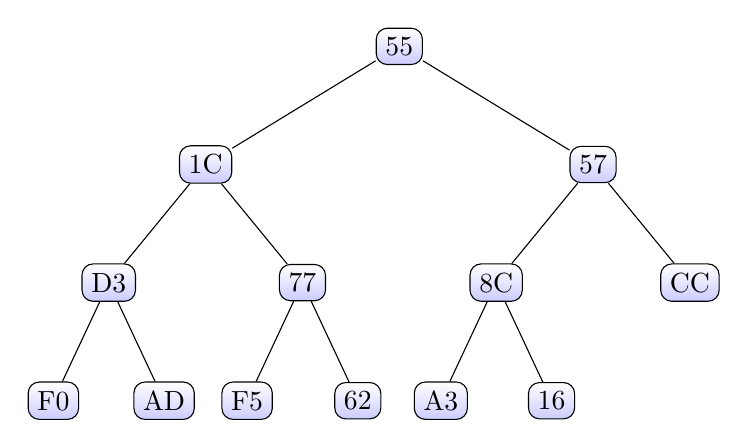
\begin{tikzpicture}[
  level 1/.style={sibling distance=14em},
  level 2/.style={sibling distance=7em},
  level 3/.style={sibling distance=4em},
  level 4/.style={sibling distance=1em}, 
  every node/.style = {shape=rectangle, rounded corners, draw, 
    align=center, top color=white, bottom color=blue!20}
  ]
  \node {55}
    child { node {1C} 
      child { node {D3}
        child { node {F0} }
        child { node {AD} }
      }
      child { node {77}
        child { node {F5} }
        child { node {62} }
      }
    } 
    child { node {57}
      child { node {8C}
        child { node {A3} }
        child { node {16} }
      }
      child { node {CC} }
    }; 
\end{tikzpicture}

\subsubsection{Proof for the first leaf}
It is clear that the proof 
\[(AD, 77, 57)\]
that the Merkle hash subtree for the first
leaf \(F0\) only is identical to the audit proof of this 
leaf.

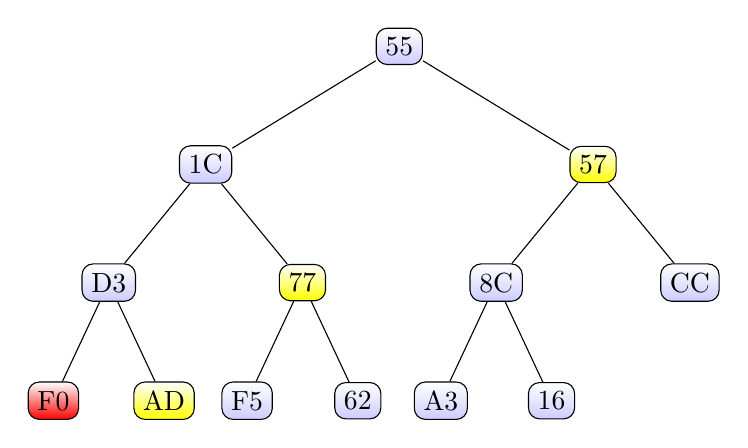
\begin{tikzpicture}[
  level 1/.style={sibling distance=14em},
  level 2/.style={sibling distance=7em},
  level 3/.style={sibling distance=4em},
  level 4/.style={sibling distance=1em}, 
  every node/.style = {shape=rectangle, rounded corners, draw, 
    align=center, top color=white, bottom color=blue!20}
  ]
  \node {55}
    child { node {1C} 
      child { node {D3}
        child { node[bottom color=red] {F0} }
        child { node[bottom color=yellow] {AD} }
      }
      child { node[bottom color=yellow] {77}
        child { node {F5} }
        child { node {62} }
      }
    } 
    child { node[bottom color=yellow] {57}
      child { node {8C}
        child { node {A3} }
        child { node {16} }
      }
      child { node {CC} }
    }; 
\end{tikzpicture}


\subsubsection{Proof for the first two leaves}
The proof for the Merkle hash subtree 

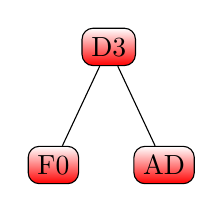
\begin{tikzpicture}[
  level 1/.style={sibling distance=4em},
  every node/.style = {shape=rectangle, rounded corners, draw, 
    align=center, top color=white, bottom color=red}
  ]
  \node {D3}
        child { node[bottom color=red] {F0} }
        child { node[bottom color=red] {AD} };
\end{tikzpicture}

of 
\((F0, AD)\)
is
\((77, 57).\)

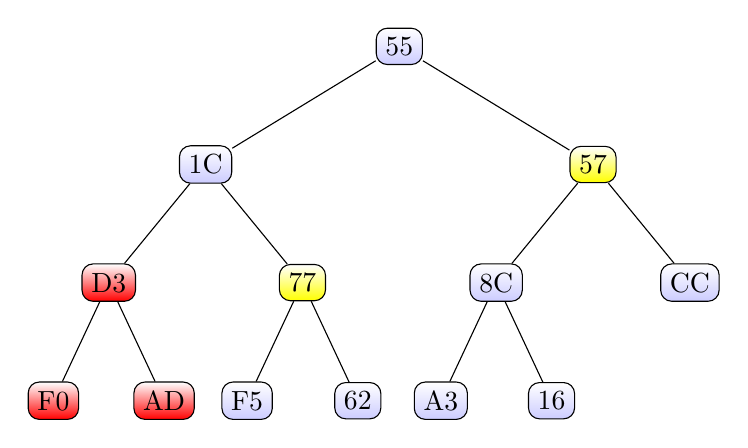
\begin{tikzpicture}[
  level 1/.style={sibling distance=14em},
  level 2/.style={sibling distance=7em},
  level 3/.style={sibling distance=4em},
  level 4/.style={sibling distance=1em}, 
  every node/.style = {shape=rectangle, rounded corners, draw, 
    align=center, top color=white, bottom color=blue!20}
  ]
  \node {55}
    child { node {1C} 
      child { node[bottom color=red] {D3}
        child { node[bottom color=red] {F0} }
        child { node[bottom color=red] {AD} }
      }
      child { node[bottom color=yellow] {77}
        child { node {F5} }
        child { node {62} }
      }
    } 
    child { node[bottom color=yellow] {57}
      child { node {8C}
        child { node {A3} }
        child { node {16} }
      }
      child { node {CC} }
    }; 
\end{tikzpicture}

\subsubsection{Proof for the first three leaves}
The proof for the Merkle hash subtree 

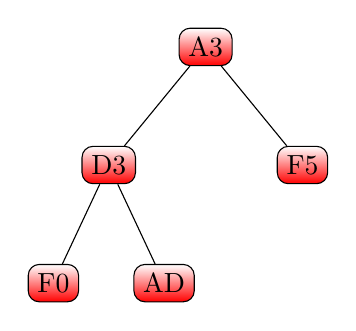
\begin{tikzpicture}[
  level 1/.style={sibling distance=7em},
  level 2/.style={sibling distance=4em},
  level 3/.style={sibling distance=1em},
  every node/.style = {shape=rectangle, rounded corners, draw, 
    align=center, top color=white, bottom color=red}
  ]
  \node {A3}
    child { node {D3} 
      child { node {F0} }
      child { node {AD} }
    }
    child { node{F5}
    }; 
\end{tikzpicture}

of 
\((F0, AD, F5)\)
is
\((F5, 62, D3, 57).\)

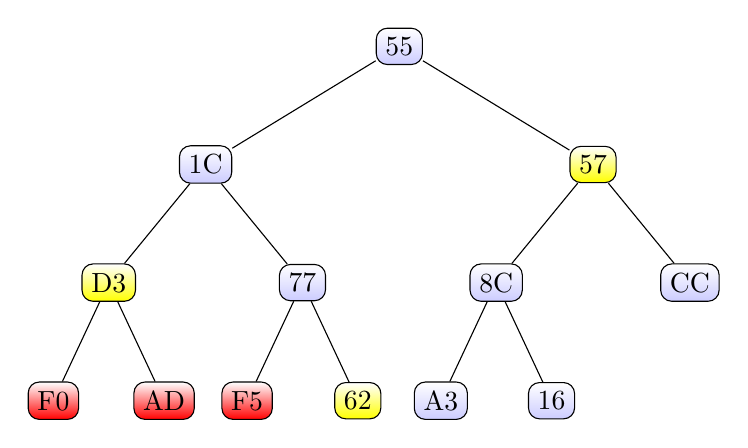
\begin{tikzpicture}[
  level 1/.style={sibling distance=14em},
  level 2/.style={sibling distance=7em},
  level 3/.style={sibling distance=4em},
  level 4/.style={sibling distance=1em}, 
  every node/.style = {shape=rectangle, rounded corners, draw, 
    align=center, top color=white, bottom color=blue!20}
  ]
  \node {55}
    child { node {1C} 
      child { node[bottom color=yellow] {D3}
        child { node[bottom color=red] {F0} }
        child { node[bottom color=red] {AD} }
      }
      child { node{77}
        child { node[bottom color=red]  {F5} }
        child { node[bottom color=yellow]  {62} }
      }
    } 
    child { node[bottom color=yellow] {57}
      child { node {8C}
        child { node {A3} }
        child { node {16} }
      }
      child { node {CC} }
    }; 
\end{tikzpicture}

\subsubsection{Proof for the first four leaves}
The proof for the Merkle hash subtree 

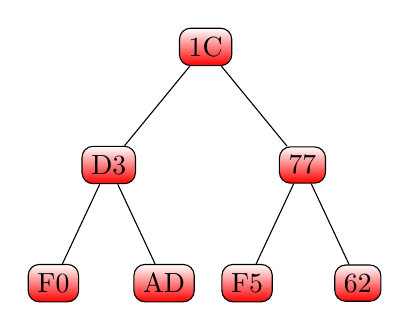
\begin{tikzpicture}[
  level 1/.style={sibling distance=7em},
  level 2/.style={sibling distance=4em},
  level 3/.style={sibling distance=1em},
  every node/.style = {shape=rectangle, rounded corners, draw, 
    align=center, top color=white, bottom color=red}
  ]
    \node {1C} 
      child { node {D3}
        child { node{F0} }
        child { node{AD} }
      }
      child { node{77}
        child { node{F5} }
        child { node{62} }
      }
    ; 
\end{tikzpicture}

of 
\((F0, AD, F5, 62)\)
is
\((57).\)

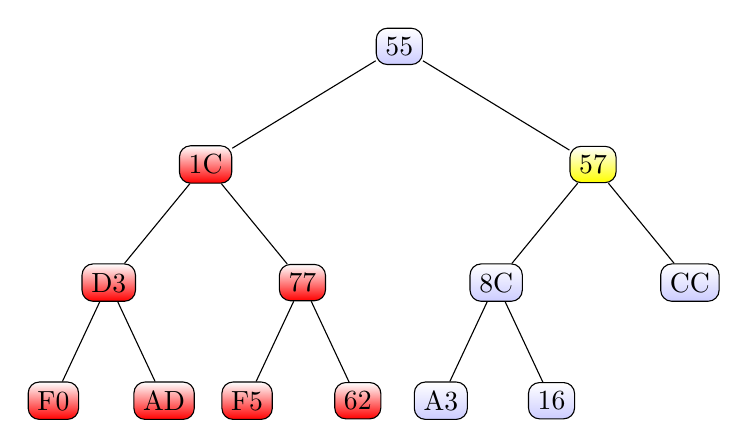
\begin{tikzpicture}[
  level 1/.style={sibling distance=14em},
  level 2/.style={sibling distance=7em},
  level 3/.style={sibling distance=4em},
  level 4/.style={sibling distance=1em}, 
  every node/.style = {shape=rectangle, rounded corners, draw, 
    align=center, top color=white, bottom color=blue!20}
  ]
  \node {55}
    child { node[bottom color=red] {1C} 
      child { node[bottom color=red] {D3}
        child { node[bottom color=red] {F0} }
        child { node[bottom color=red] {AD} }
      }
      child { node[bottom color=red]{77}
        child { node[bottom color=red]  {F5} }
        child { node[bottom color=red]  {62} }
      }
    } 
    child { node[bottom color=yellow] {57}
      child { node {8C}
        child { node {A3} }
        child { node {16} }
      }
      child { node {CC} }
    }; 
\end{tikzpicture}


\subsubsection{Proof for the first five leaves}
The proof for the Merkle hash subtree 

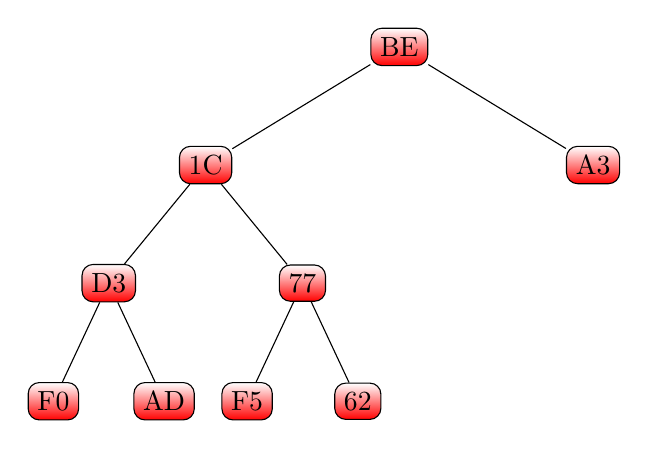
\begin{tikzpicture}[
  level 1/.style={sibling distance=14em},
  level 2/.style={sibling distance=7em},
  level 3/.style={sibling distance=4em},
  level 4/.style={sibling distance=1em},
  every node/.style = {shape=rectangle, rounded corners, draw, 
    align=center, top color=white, bottom color=red}
  ]
  \node {BE}
    child { node{1C} 
      child { node{D3}
        child { node{F0} }
        child { node{AD} }
      }
      child { node {77}
        child { node{F5} }
        child { node{62} }
      }
    } 
    child { node{A3}
    }; 
\end{tikzpicture}

of 
\((F0, AD, F5, 62, A3)\)
is
\((A3, 16, CC, 1C).\)

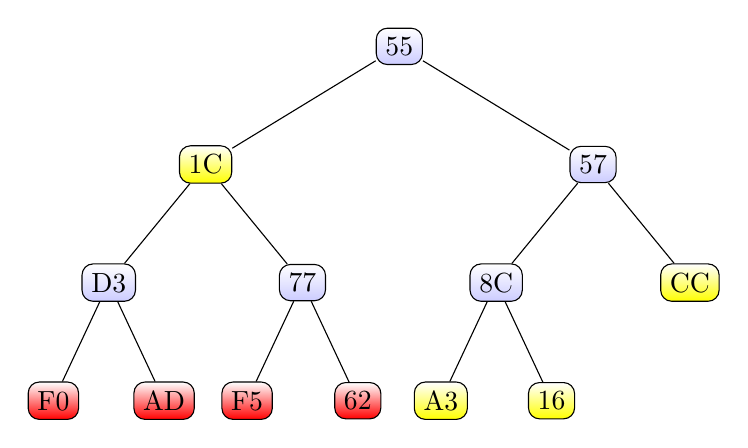
\begin{tikzpicture}[
  level 1/.style={sibling distance=14em},
  level 2/.style={sibling distance=7em},
  level 3/.style={sibling distance=4em},
  level 4/.style={sibling distance=1em}, 
  every node/.style = {shape=rectangle, rounded corners, draw, 
    align=center, top color=white, bottom color=blue!20}
  ]
  \node {55}
    child { node[bottom color=yellow] {1C} 
      child { node{D3}
        child { node[bottom color=red] {F0} }
        child { node[bottom color=red] {AD} }
      }
      child { node {77}
        child { node[bottom color=red]  {F5} }
        child { node[bottom color=red]  {62} }
      }
    } 
    child { node{57}
      child { node {8C}
        child { node[bottom color=yellow] {A3} }
        child { node[bottom color=yellow] {16} }
      }
      child { node[bottom color=yellow] {CC} }
    }; 
\end{tikzpicture}

\subsubsection{Proof for the first six leaves}
The proof for the Merkle hash subtree 

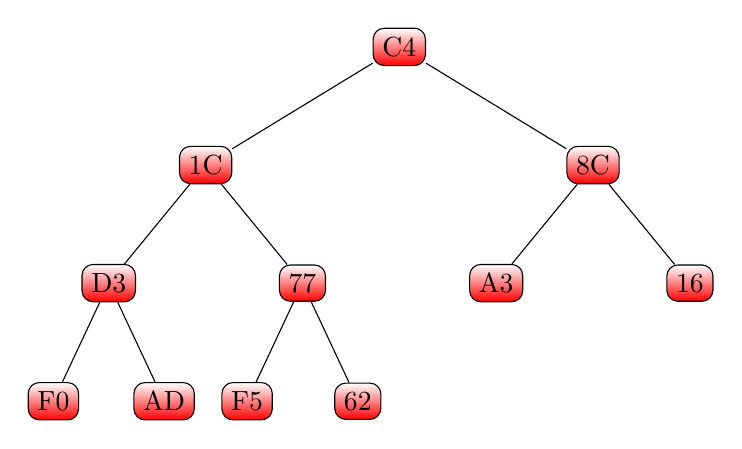
\begin{tikzpicture}[
  level 1/.style={sibling distance=14em},
  level 2/.style={sibling distance=7em},
  level 3/.style={sibling distance=4em},
  level 4/.style={sibling distance=1em},
  every node/.style = {shape=rectangle, rounded corners, draw, 
    align=center, top color=white, bottom color=red}
  ]
  \node {C4}
    child { node{1C} 
      child { node{D3}
        child { node{F0} }
        child { node{AD} }
      }
      child { node {77}
        child { node{F5} }
        child { node{62} }
      }
    } 
    child { node{8C}
        child { node{A3} }
        child { node{16} }
    }; 
\end{tikzpicture}

of 
\((F0, AD, F5, 62, A3, 16)\)
is
\((8C, CC, 1C).\)

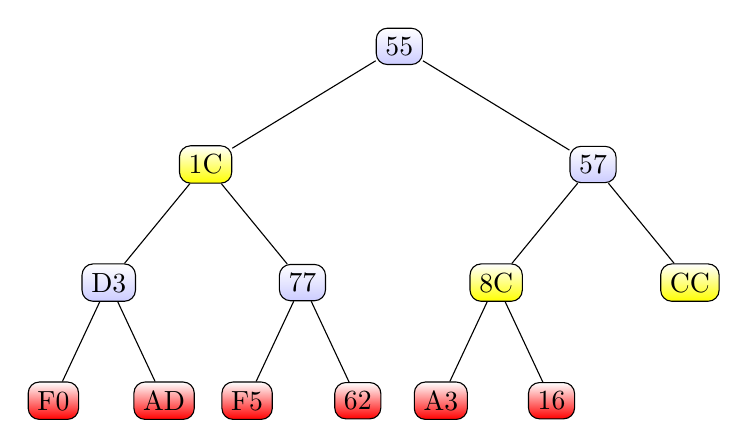
\begin{tikzpicture}[
  level 1/.style={sibling distance=14em},
  level 2/.style={sibling distance=7em},
  level 3/.style={sibling distance=4em},
  level 4/.style={sibling distance=1em}, 
  every node/.style = {shape=rectangle, rounded corners, draw, 
    align=center, top color=white, bottom color=blue!20}
  ]
  \node {55}
    child { node[bottom color=yellow] {1C} 
      child { node{D3}
        child { node[bottom color=red] {F0} }
        child { node[bottom color=red] {AD} }
      }
      child { node {77}
        child { node[bottom color=red]  {F5} }
        child { node[bottom color=red]  {62} }
      }
    } 
    child { node{57}
      child { node[bottom color=yellow] {8C}
        child { node[bottom color=red] {A3} }
        child { node[bottom color=red] {16} }
      }
      child { node[bottom color=yellow] {CC} }
    }; 
\end{tikzpicture}



